\documentclass{article}
\usepackage{fancyhdr}
\usepackage{tikz}
\pagestyle{fancy}
\setlength{\headheight}{35pt}
\lhead{Distributed System I\\Wintersemester2020/21\\Assignment 5}
\chead{}
% bfseries
\rhead{Ciheng Zhang (3472321)\\Chenxi Li(3502796)\\Yaosheng Zheng (3563285)\\Leqi Xu(3556962)}
\cfoot{\thepage}
\renewcommand{\headrulewidth}{0.4pt}

\begin{document}
\begin{titlepage}
    \title{\Huge \textbf{Distributed System I\\Wintersemester2020/21\\Assignment 5} }
    \author{\LARGE \textsl{Ciheng Zhang (3472321) zch3183505@gmail.com}\\\LARGE \textsl{Chenxi Li(3502796) cli216@outlook.com }\\\LARGE \textsl{Leqi Xu(3556962) st176119@stud.uni-stuttgart.de} \\\LARGE \textsl{Yaosheng Zheng (3563285) zhengyaosheng312@icloud.com}\\\LARGE \textsl{Team 19 } \\[200pt]}
    \date{\today}
    \maketitle
    \thispagestyle{empty}
\end{titlepage}
\newpage
\section{Two-Phase Locking}
\subsection*{a)}
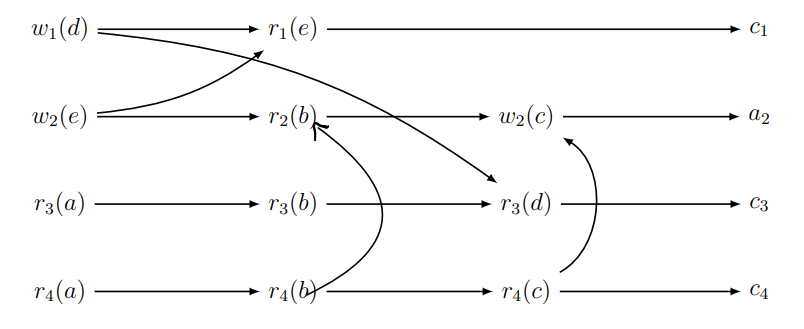
\includegraphics{01.png}
The missing way is in the figure.
\newpage
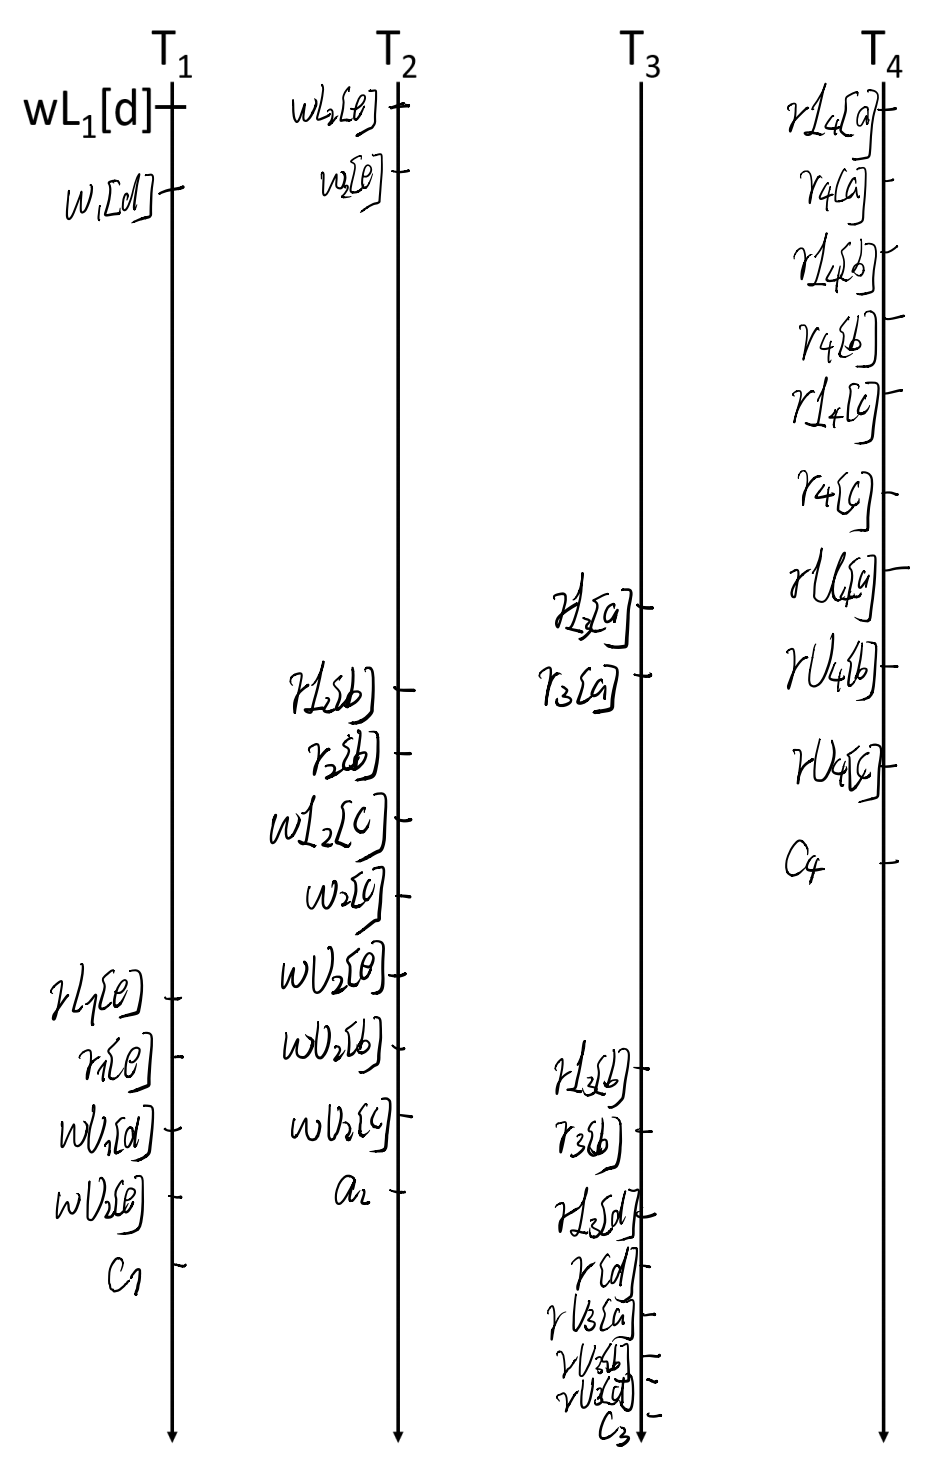
\includegraphics[scale=0.7]{02.png}
\newpage
\subsection*{b)}
T1 have to abort.\\ Because $w_2(2)->r_1(e)$. So the value of T2 affects T1.
\subsection*{c)}
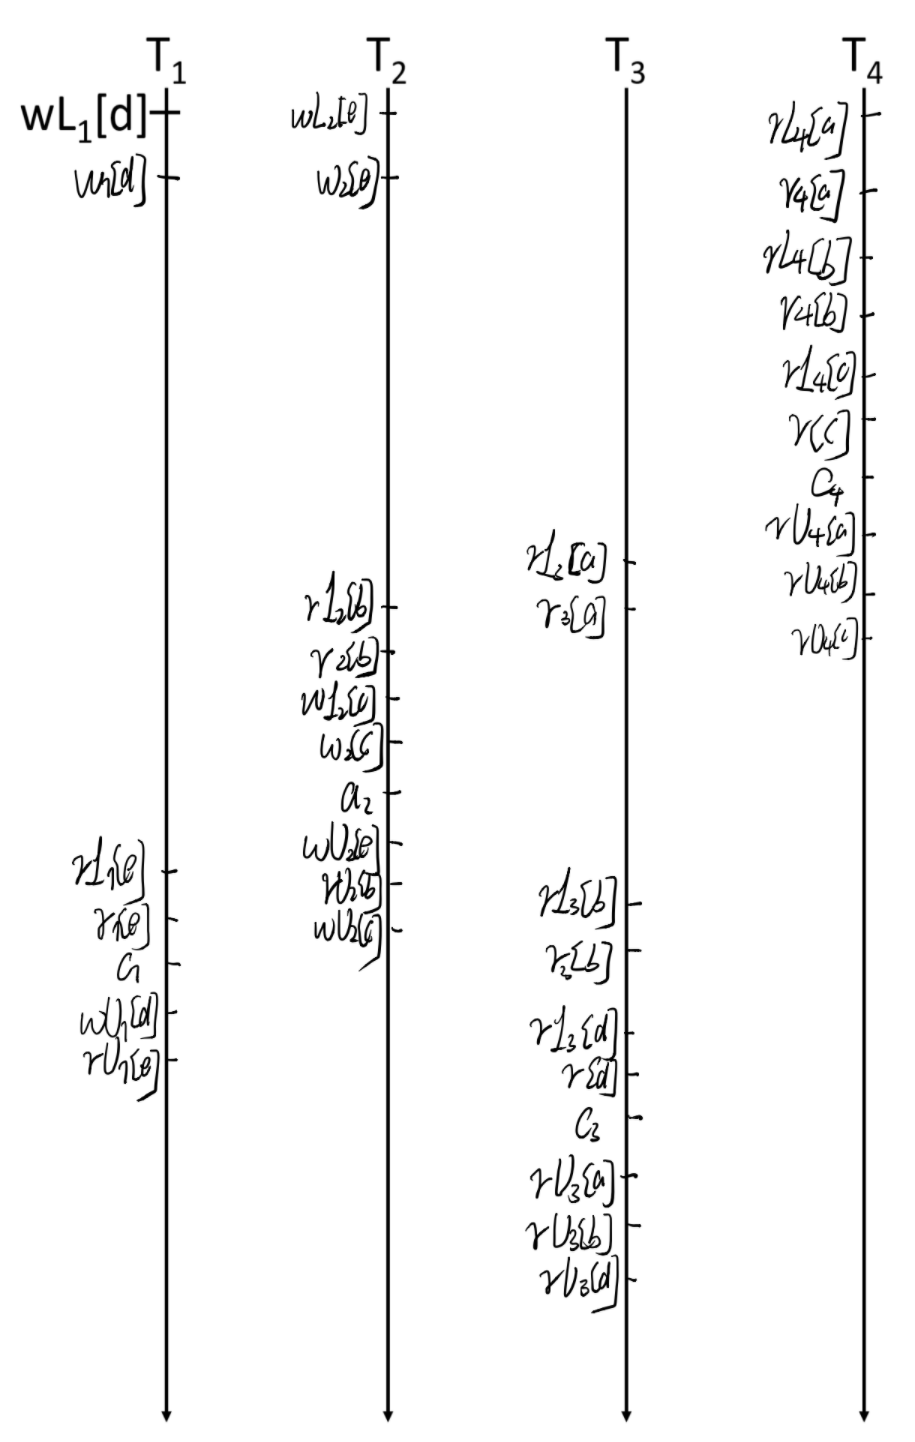
\includegraphics[scale=0.6]{03.png}
\section{Two-Phase Commit}
\subsection*{a)}
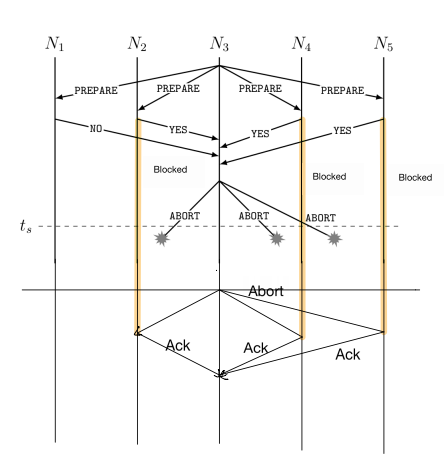
\includegraphics[scale=0.8]{04.png}
 $N_1$ dont need to wait.
 \subsection*{b)}
  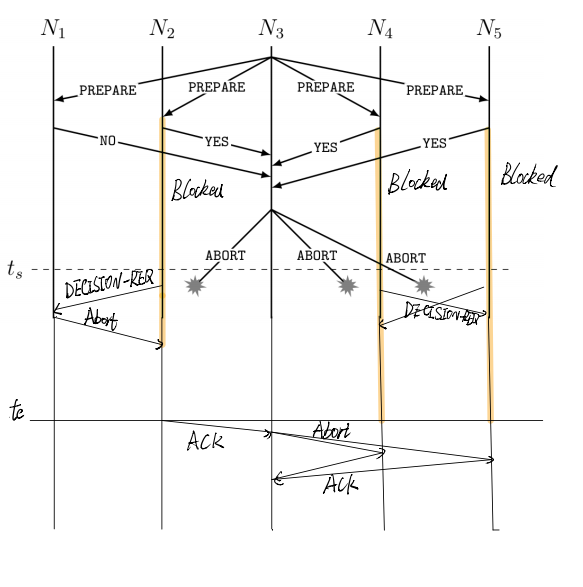
\includegraphics[scale=0.8]{05.png}
  \\when N2,N4,N5 is time out. Then they send DECISION-REQ to others. In this situation N4,N5 send to each other. N2 send to N1
  N1 know should be Abort and send Abort to N2. Then N2 is unblocked. After $t_e$ send a ACK to N3. By N4 and N5 both of them 
  dont know COMMIT or ABORT. So they still be blocked until recive a ABORT message from N3.
  \subsection*{c)}
  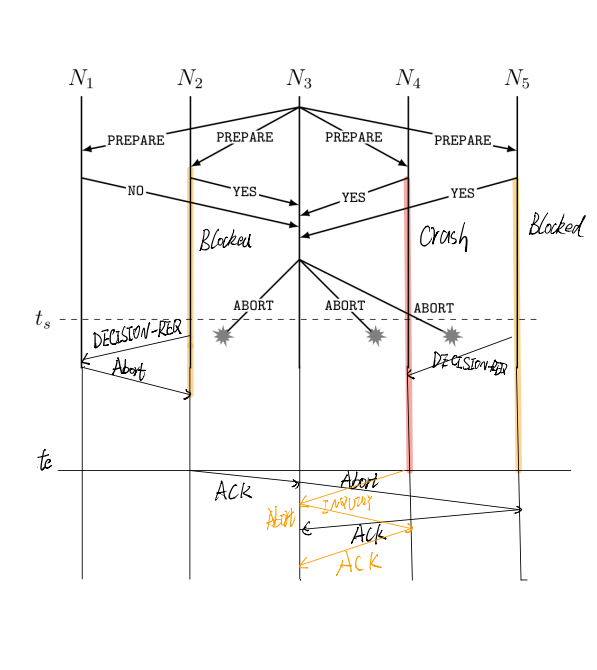
\includegraphics{06.png}
  \\After crash N4 send a INQUIRY message to N3 and N3 send back a ABORT message. Then N4 send back a ACK.

  \section{Data Replication}
\subsection*{a)}
The Assume is  A: 5, B:1, C:1, D:1.
\\ The write quorums and read quorums are:
\\\{A\},\{A,B\},\{A,B,C\},\{A,B,C,D\}
\\Because $q_r[X]+ q_w[X]>q[X]$ and $q_w[X]>q[X]/2$. So $q[X]<9$. And we want to minmizes the number of nodes. So we need to make 
one Note that can direct bigger than threshold. So one Note have weight 5. And every Node at least have 1 and total number smaller 
than 9. So $q[X]=8$ node A is 5 others is 1. 
\\ In this Assume, Only need to lock A.
\subsection*{b)}
A:3,B:3,C:1,D:1
\\
 We want to maximal the availabity.So we need to assign weight by availabity.and dont allow only one node can bigger thean threshold.
 The write quorums is:
 \\\{A,B\},\{A,B,C\},\{A,B,C,D\},\{A,B,D\},\{A,C,D\},\{B,C,D\}
 \\The read quorums is:
 \\\{A,B\},\{A,C\},\{A,D\},\{A,B,C\},\{A,B,D\},\{A,C,D\},\{A,B,C,D\},\{B,C\},\{B,D\},\{B,C,D\}
 \\In this Assume only A and B both have failure will cause a not available state.
 
\subsection*{c)}
$q_w[X]=6$
\\The write quorums are:
\\\{A,B\},\{A,B,C\},\{A,B,C,D\},\{A,B,D\},\{A,C,D\},\{B,C,D\}
\subsection*{d)}
By Majority Consensus methode in this situation must have 2 votes. So the tolerates is two node failure.
This mean, K ,L or K,M or L,M or L,K,M have failure the Y is not available for reading. The term is:
\[P_r(Y)=1-(1-p_K)(1-p_L)-(1-p_K)(1-p_M)-(1-p_L)(1-p_M)-(1-p_K)(1-p_L)(1-p_M)\]
\end{document}
